% !Mode::"TeX:UTF-8"
% \documentclass[twocolumn,landscape,UTF8]{ctexart}
\documentclass[twocolumn,landscape]{article}
\usepackage[UTF8]{ctex}
\usepackage{lastpage}
%\usepackage{times} %use the Times New Roman fonts
\usepackage{color}
%\usepackage{placeins}
\usepackage{ulem}
\usepackage{titlesec}
\usepackage{graphicx}
\usepackage{colortbl}
\usepackage{listings}
\usepackage{makecell}
\usepackage{indentfirst}
\usepackage{fancyhdr}
\usepackage{setspace} % 行间距
\usepackage{bm}%\boldsymbol 粗体
% 数学
\usepackage{amsmath,amsfonts,amsmath,amssymb,times}
\usepackage{txfonts}
\usepackage{enumerate}% 编号
\usepackage{tikz,pgfplots} %绘图
\usepackage{tkz-euclide,pgfplots}
\usetikzlibrary{automata,positioning}
%\usepackage[paperwidth=18.4cm,paperheight=26cm,top=1.5cm,bottom=2cm,right=2cm]{geometry} % 单页
\usepackage[paperwidth=36.8cm,paperheight=26cm,top=2.5cm,bottom=2cm,right=2cm]{geometry}
\lstset{language=C,keywordstyle=\color{red},showstringspaces=false,rulesepcolor=\color{green}}
\oddsidemargin=0.5cm   %奇数页页边距
\evensidemargin=0.5cm %偶数页页边距
%\textwidth=14.5cm        %文本的宽度 单页
\textwidth=30cm        %文本的宽度 单页

\newsavebox{\zdx}%装订线

\newcommand{\putzdx}{\marginpar{
		\parbox{1cm}{\vspace{-1.6cm}
			\rotatebox[origin=c]{90}{
				\usebox{\zdx}
		}}
}}

\newcommand{\blank}{\uline{\textcolor{white}{a}\ \textcolor{white}{a}\ \textcolor{white}{a}\ \textcolor{white}{a}\ \textcolor{white}{a}\ \textcolor{white}{a}\ \textcolor{white}{a}\ \textcolor{white}{a}\ \textcolor{white}{a}\ \textcolor{white}{a}\ \textcolor{white}{a}}}

\newcommand{\me}{\mathrm{e}}  %定义 对数常数e,虚数符号i,j以及微分算子d为直立体。
\newcommand{\mi}{\mathrm{i}}
\newcommand{\mj}{\mathrm{j}}
\newcommand{\dif}{\mathrm{d}}
\newcommand{\bs}{\boldsymbol}%数学黑体
\newcommand{\ds}{\displaystyle}
%通常我们使用的分数线是系统自己定义的分数线,即分数线的长度的预设值是分子或分母所占的最大宽度,如何让分数线的长度变长成,我们%可以在分子分母添加间隔来实现。如中文分式的命令可以定义为:
%\newcommand{\chfrac[2]}{\cfrac{\;#1\;}{\;#2\;}}
%\frac{1}{2} \qquad \chfrac{1}{2}

%选择题
\newcommand{\fourch}[4]{\\\begin{tabular}{*{4}{@{}p{3.5cm}}}A.~#1 & B.~#2 & C.~#3 & D.~#4\end{tabular}} % 四行
\newcommand{\twoch}[4]{\\\begin{tabular}{*{2}{@{}p{7cm}}}A.~#1 & B.~#2\end{tabular}\\\begin{tabular}{*{2}{@{}p{7cm}}}C.~#3 &
		D.~#4\end{tabular}}  %两行
\newcommand{\onech}[4]{\\A.~#1 \\ B.~#2 \\ C.~#3 \\ D.~#4}  % 一行

\renewcommand{\headrulewidth}{0pt}
\pagestyle{fancy}
\begin{document} % 在begin前面加了一个空格以免出现显示错误,编译时应该去掉
\fancyhf{}
\fancyfoot[CO,CE]{\vspace*{1mm}第\,\thepage\,页 , 共2页}
\sbox{\zdx}
{\parbox{27cm}{\centering
	座位号~\underline{\makebox[34mm][c]{}}~ 班~级\underline{\makebox[34mm][c]{}}~\CJKfamily{song} 学~号\underline{\makebox[44mm][c]{}}~\CJKfamily{song} 姓~名\underline{\makebox[34mm][c]{}} ~\\
	\vspace{3mm}
请在所附答题纸上空出密封位置。并填写试卷序号、班级、学号和 姓名\\
%答题时学号
\vspace{1mm}
\dotfill{} 密\dotfill{}封\dotfill{}线\dotfill{} \\
	}}
	\reversemarginpar
	
\begin{spacing}{1.25}
	\begin{center}
\begin{LARGE}
~\underline{~2021 }\,年普通高等学校招生全国统一考试\\
\underline{数学}\,试卷\\
\end{LARGE}
(笔试\ \ 120 分钟)\\
%	\vspace{0.5cm}

\end{center}
\end{spacing}
%\vspace{-0.5cm}
\setlength{\marginparsep}{1.7cm}
\putzdx %%装订线--奇页数
%\vspace{1cm}

  
\section*{一、单选题~(每题~5 分,共~40 分)}	
\begin{enumerate}\setcounter{enumi}{0}

\item 设集合~$A=\{x \mid-2<x<4\}$,$B = \{2,3,4,5\}$ ,则~$A\cap B=$~( ~~ )
\fourch{$\{2\}$}{$\{2,3\}$}{$\{3,4\}$}{$\{2,3,4\}$}

\item 已知$z=2-i$,则$(z(\vec{z}+i))=$~( ~~ )
\fourch{$6-2i$}{$4-2i$}{$6+2i$}{$4+2i$}

%\onech{分段函数一定不是初等函数.}{若 $\lim\limits_{n\rightarrow \infty}x_ny_n=0$, 则必有 $\lim\limits_{n\rightarrow \infty}x_n=0$ 或 $\lim\limits_{n\rightarrow \infty}y_n=0$.}{若 $f(x)$ 在 $(a,b) $ 内连续,则$f(x)$ 在 $(a,b) $ 内必有界.}{若$\lim\limits_{n\rightarrow \infty}x_n=a$($a$ 为有限实数),则数列 $\{x_n\}$ 必有界.}

\item 已知圆锥的底面半径为$\sqrt2$,其侧面展开图为一个半圆,则该圆锥的母线长为~( ~~ )
\fourch{$2$}{$2\sqrt2$}{$4$}{$4\sqrt2$}
			
\item 下列区间中,函数$f(x)=7 \sin \left(x-\frac{\pi}{6}\right)$单调递增的区间是~( ~~ )
\fourch{$\left(0, \frac{\pi}{2}\right)$}{$\left(\frac{\pi}{2}, \pi\right)$}{$\left(\pi, \frac{3\pi}{2}\right)$}{$\left(\frac{3\pi}{2}, 2\pi\right)$}

\item 已知$F_1$,$F_2$是椭圆$C$:$\frac{x^2}{9}+\frac{y^2}{4}=1$的两个焦点,点$M$在$C$上,则$\left|\mathrm{MF}_{1}\right| \cdot\left|\mathrm{MF}_{2}\right|$的最大值为~( ~~ )
\fourch{$13$}{$12$}{$9$}{$6$}

\item 若$\tan \theta=-2$,则$\frac{\sin{\theta\left(1+\sin{2\theta}\right)}}{\sin{\theta}+\cos{\theta}}$ =~( ~~ )
\fourch{$-\frac{6}{5}$}{$-\frac{2}{5}$}{$\frac{6}{5}$}{$\frac{2}{5}$}

\item 若过点$(a,b)$可以作曲线$ y=e^{x} $的两条切线,则~( ~~ )
\onech{$\mathrm{e}^{\mathrm{b}}<\mathrm{a}$}{$\mathrm{e}^{\mathrm{a}}<\mathrm{b}$}{$0<\mathrm{a}<\mathrm{e}^{\mathrm{b}}$}{$0<\mathrm{b}<\mathrm{e}^{\mathrm{a}}$}

\item 有6个相同的球,分别标有数字1,2,3,4,5,6,从中有放回的随机取两次,每次取1个球,甲表示事件“第一次取出的球的数字是1”,乙表示事件“第二次取出的球的数字是2”,丙表示事件“两次取出的球的数字之和是8”,丁表示事件“两次取出的球的数字之和是7”,则~( ~~ )
\onech{$\mbox{甲与丙相互独立}$}{$\mbox{甲与丁相互独立}$}{$\mbox{乙与丙相互独立}$}{$\mbox{丙与丁相互独立}$}

\end{enumerate}
%\newpage
\section*{二、多选题~(每题~5 分,共~20 分)}
%\vspace{-1cm}
\textbf{全部选对的得5分,部分选对的得2分,有选错的得0分。}

\begin{enumerate}\setcounter{enumi}{8}
			
\item 有一组样本数据$ x_{1}, x_{2},\cdots,x_{n} $,由这组数据得到新样本数据$ y_{1}, y_{2},\cdots,y_{n} $,其中$y_{i}=x_{i}+c~(i=1,2, \cdots, n) $, $c$为非零常数,则~( ~~ )
\onech{\mbox{两组样本数据的样本平均数相同}}{\mbox{两组样本数据的样本中位数相同}}{\mbox{两组样本数据的样本标准差相同}}{\mbox{两组样本数据的样本极差相同}}

\item 已知$O$为坐标原点,点$P_1(\cos\alpha,sin\alpha)$,~$P_2(cos\beta,-sin\beta)$,~$P_3(cos(\alpha+\beta),sin(\alpha+\beta))$,$A(1,0)$,则~( ~~ )
\twoch{$\mid \overrightarrow{\mathrm{OP}_1}\mid=\mid \overrightarrow{\mathrm{OP}_2}\mid$}{$\mid\overrightarrow{\mathrm{AP}_1}\mid=\mid \overrightarrow{\mathrm{AP}_2}\mid$}{$\overrightarrow{\mathrm{OA}}\cdot\overrightarrow{\mathrm{OP}_3}=\overrightarrow{\mathrm{OP}_1}\cdot\overrightarrow{\mathrm{OP}_2}$}{$\overrightarrow{\mathrm{OA}}\cdot\overrightarrow{\mathrm{OP}_1}=\overrightarrow{\mathrm{OP}_2}\cdot\overrightarrow{\mathrm{OP}_3}$}

\item 已知点$P$在圆${(x-5)}^2+ {(y-5)}^2 =16$上,点$A(4,0)$,$B(0,2)$,则~( ~~ )
\onech{$\mbox{点$P$到直线$AB$的距离小于10}$}{$\mbox{点$P$到直线$AB$的距离大于2}$}{$\mbox{当$\angle\mathrm{PBA}$最小时,$\mid\mathrm{PB}\mid=3\sqrt{2}$}$}{$\mbox{当$\angle\mathrm{PBA}$最大时,$\mid\mathrm{PB}\mid=3\sqrt{2}$}$}

\item 在正三棱柱 $ABC-A_1B_1C_1$中,$AB=AA_1=1$,点 $P$ 满足$\overrightarrow{PB}=\lambda\overrightarrow{BC}+\mu\overrightarrow{BB_1}$,其中$\lambda\in[0,1]$,~$\mu\in[0,1]$ , 则~( ~~ )
\onech{$\mbox{点$P$到直线$AB$的距离小于10}$}{$\mbox{点$P$到直线$AB$的距离大于2}$}{$\mbox{当$\angle\mathrm{PBA}$最小时,$\mid\mathrm{PB}\mid=3\sqrt{2}$}$}{$\mbox{当$\mu=\frac{1}{2}$时,有且仅有一个点 $P$, 使得$A_{1}B\perp\text{平面} AB_{1}P$}$}

\end{enumerate}

%\vspace{2cm}
\section*{ 三、填空题~(每题~5 分, 共~20 分)}
%\vspace{-1cm}

		\begin{enumerate}\setcounter{enumi}{12}
			\item 已知函数 $f(x)=x^3(a\cdot2^x-2^{-x})$是偶函数,则 $a$=\underline{~~~~}.
			
			\item 已知$O$为坐标原点,抛物线$C$:$\mathrm{y^2= 2px( p> 0) }$ 的焦点为$F$,$P$为$C$上一点,$PF$与$x$轴垂直,$Q$为$x$ 轴上一点,且$PQ\perp OP$,若$\mid FQ\mid =6$, 则$C$的准线方程为\underline{~~~~~~}.
			
			\item 函数$f(x)=\mid {2x-1}\mid-2\ln{x}$的最小值为\underline{~~~~~~}.
   
			\item 某校学生在研究民间剪纸艺术时,发现此纸时经常会沿纸的某条对称轴把纸对折.规格为$20\mathrm{dm}\times 12\mathrm{dm}$ 的长方形纸.对折 1 次共可以得到 $10\mathrm{dm}\times 2\mathrm{dm}$,~ $20\mathrm{dm}\times 6\mathrm{dm}$ 两种规格的图形,它们的面积之和$S_1=240 \mathrm{dm}^2$,对折 2 次共可以得 $5\mathrm{dm}\times 12\mathrm{dm}$ ,~ $10\mathrm{dm}\times 6\mathrm{dm}$,~ $20\mathrm{dm}\times 3\mathrm{dm}$ 三种规格的图形,它们的面积之和$S_{2}=180\mathrm{dm}^{2}$.以此类推,则对折 4 次共可以得到不同规格图形的种数为\underline{~~~~~~}.如果对折$n$ 次,那么$\sum_{k=1}^{n}S_k$= \underline{~~~~~~}.
			
		\end{enumerate}
		
		%\newpage
		\putzdx %%装订线--奇页数
		
		\section*{四、解答题~(共~70分)}
		%\vspace{-2cm}

		\begin{enumerate}\setcounter{enumi}{16}
		\item (10 分)已知数列{$a_n$}满足$a_1=1,\quad a_{n+1}\begin{cases}a_n+1,&\mbox{n为奇数}\\a_n+2,&\mbox{n为偶数}\end{cases}$
  
  (1)记$b_n=a_{2n}$, 写出$b_1,b_2$,并求数列$\{b_n\}$的通项公式;
  
  (2)求$\{a_n\}$的前 20 项和
  
\vspace{1.5cm}
		

\item  (12 分)

某学校组织"一带一路”知识竞赛,有A,B两类问题・每位参加比赛的同学先在两类问题中选择类并从中随机抽取一个问题回答,若回答错误则该同学比赛结束;若 回答正确则从另一类问题中再随机抽取一个问題回答,无论回答正确与否,该同学比赛 结束.A类问题中的每个问题回答正确得20分,否则得0分:B类问题中的每个问题 回答正确得80分,否则得0分。

己知小明能正确回答A类问题的概率为0.8 ,能正确回答B类问題的概率为0.6 . 且能正确回答问题的概率与回答次序无关。

(1)若小明先回答A类问题,记$X$为小明的累计得分,求$X$的分布列:

(2)为使累计得分的期望最大,小明应选择先回答哪类问题?并说明理由。

\vspace{1.5cm}

\item  (12 分)

记 $\bigtriangleup ABC$ 的内角 $A$, $B$, $C$ 的对边分别为 $a$, $b$, $c$, 已知$b^2 = ac$, 点 $D$ 在边 $AC$ 上,$BD \sin{\angle ABC}~=~a\sin{C}$

(1)证明:$BD = b$.

(2)若 $AD = 2DC$ . 求 $\cos{\angle ABC}$.

\vspace{1.5cm}
\newpage

\item  (12 分)

如图\ref{20-fig},在三棱锥$A-BCD$中,$\text{平面}ABD\perp \text{平面}BCD$,$AB=AD$,$O$为$BD$的中点.

(1)证明:$OA \perp CD$.

(2)若$\bigtriangleup OCD$是边长为1的等边三角形.点$E$在棱$AD$上. $DE = 2EA$ .且二面角$E-BC-D$的大小为45°,求三棱锥$A-BCD$的体积.

\begin{figure}[h]
	\centering
	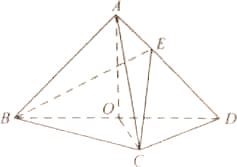
\includegraphics[width=0.1\textwidth]{20.png}
	\caption{三棱锥$A-BCD$}
	\label{20-fig}
\end{figure}

\vspace{2cm}

\item  (12 分)

在平面直角坐标系 $xOy$ 中,己知点$F_1(-\sqrt{17},0)$, $F_2(\sqrt{17},0)$,点 $M$ 满足$\mid MF_{1}\mid -\mid MF_{2}\mid =2$,记 $M$ 的轨迹为$C$.

(1)求$C$的方程.

(2)设点 $T$ 在直线$x=\frac{1}{2}$上,过 $T$ 的两条直线分别交 $C$ 于 $A$, $B$ 两点和 $P$, $Q$ 两点,且$\mid TA\mid \cdot \mid TB \mid = \mid TP\mid \cdot \mid TQ \mid$ ,求直线 $AB$ 的斜率与直线 $PQ$ 的斜率之和.

\vspace{2cm}

\item   (12 分)

已知函数 $f(x) = x(1-\ln{x})$

(1)讨论$f(x)$的单调性

(2)设 $a$,$b$ 为两个不相等的正数,且 $b\ln{a}-a\ln{b}=a-b$ 证明$:2<\frac1a+\frac1b<\mathrm{e}$

\end{enumerate}
%\vspace{2cm}

	\clearpage
	
\end{document}
